\chapter*{¿Dónde debería un piloto iniciar su aterrizaje?}
\begin{wrapfigure}{l}{0.35\textwidth}
	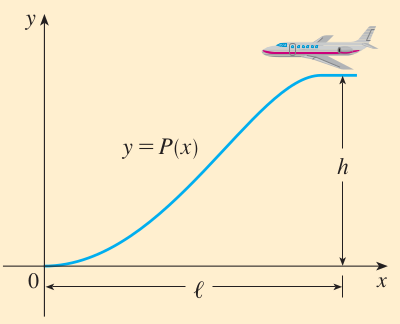
\includegraphics[width = 0.35\textwidth]{recursos/Captura desde 2024-09-21 16-53-03.png}
\end{wrapfigure}
\noindent En la figura se muestra una trayectoria de aproximación para el aterrizaje de un avión, que satisface las condiciones siguientes:

\begin{enumerate}[label=\Roman*)]
	\item La altura del crucero es $h$ cuando se inicia el descenso a una distancia $l$ del punto de contacto con la pista en el origen.
	\item El piloto debe mantener una rapidez horizontal constante $v$ a todo lo largo del descenso.
	\item El valor absoluto de la aceleración vertical no debe sobrepasar una constante $k$ (la cual es mucho menor que la aceleración debida a la gravedad).
\end{enumerate}

\begin{enumerate}
	\item Encuentre un polinomio cúbico $P(x)= ax^3+ bx^2 + cx + d$ que satisfaga la condición I),
	      imponiendo condiciones adecuadas sobre $P(x)$ y $P'(x)$ en el inicio del descenso y el contacto
	      con la pista.
	\item Use las condiciones I) y III) para demostrar que$$\frac{6hv^2}{l^2}\leq k$$
	\item Suponga que una aerolínea comercial decide no permitir que la aceleración vertical de un avión sea mayor que $k = 860 mi/h^2$. Si la altitud de crucero de un avión es de $35 000$ pies y la rapidez de $300 mi/h$, ¿a qué distancia del aeropuerto debe el piloto iniciar el descenso?
\end{enumerate}
